\documentclass[aspectratio=169,10pt]{beamer}

\usepackage[spanish]{babel}
\usepackage[utf8]{inputenc}
\usepackage[T1]{fontenc}
\usepackage{lmodern}
\usepackage{graphicx}
\usepackage{booktabs}
\usepackage{tikz}
\usepackage{ragged2e}
\usepackage{array}

\usetikzlibrary{positioning}
\setbeamertemplate{navigation symbols}{}
\setbeamertemplate{headline}{}

\definecolor{cobre}{HTML}{B55A2A}
\definecolor{cobrebrillo}{HTML}{D48A45}
\definecolor{cobreoscuro}{HTML}{6B331B}
\definecolor{mineral}{HTML}{182027}
\definecolor{carbon}{HTML}{0E1216}
\definecolor{arena}{HTML}{E8D4AD}
\definecolor{verdeoxido}{HTML}{3F6B55}
\definecolor{papel}{HTML}{F7F1E8}

\setbeamercolor{normal text}{fg=mineral,bg=white}
\setbeamercolor{frametitle}{fg=white,bg=carbon}
\setbeamerfont{frametitle}{series=\bfseries,size=\Large}
\setbeamerfont{footline}{size=\scriptsize}
\setbeamertemplate{footline}{%
  \begin{beamercolorbox}[wd=\paperwidth,ht=2.9ex,dp=1.2ex,leftskip=0.45cm,rightskip=0.45cm]{frametitle}
    \color{arena}Producción de cobre en Chile \hfill \insertframenumber/\inserttotalframenumber
  \end{beamercolorbox}
}

\newcommand{\bgphoto}[3]{%
  \begin{tikzpicture}[remember picture,overlay]
    \node[anchor=center] at (current page.center) {
      \includegraphics[width=\paperwidth,height=\paperheight]{#1}
    };
    \fill[#2,opacity=#3] (current page.south west) rectangle (current page.north east);
  \end{tikzpicture}
}

\newcommand{\copperband}{%
  \begin{tikzpicture}[remember picture,overlay]
    \fill[cobre,opacity=0.90] (current page.south west) rectangle ([yshift=0.15cm]current page.south east);
    \fill[cobrebrillo,opacity=0.85] (current page.south west) rectangle ([xshift=0.34\paperwidth,yshift=0.15cm]current page.south west);
  \end{tikzpicture}
}

\newcommand{\panel}[2]{%
  \begin{tikzpicture}
    \node[
      rounded corners=4pt,
      fill=white,
      fill opacity=0.88,
      text opacity=1,
      inner sep=8pt,
      text width=#1,
      align=left
    ] {#2};
  \end{tikzpicture}
}

\newcommand{\darkpanel}[2]{%
  \begin{tikzpicture}
    \node[
      rounded corners=4pt,
      fill=carbon,
      fill opacity=0.86,
      text opacity=1,
      inner sep=8pt,
      text width=#1,
      align=left
    ] {#2};
  \end{tikzpicture}
}

\newcommand{\metriccard}[3]{%
  \begin{tikzpicture}
    \node[
      rounded corners=5pt,
      fill=white,
      fill opacity=0.90,
      text opacity=1,
      draw=cobrebrillo,
      line width=0.7pt,
      inner sep=8pt,
      minimum height=1.55cm,
      text width=#1,
      align=left
    ] {
      {\color{cobreoscuro}\scriptsize\bfseries #2}\\[-1pt]
      {\color{mineral}\Large\bfseries #3}
    };
  \end{tikzpicture}
}

\newcommand{\slidetitle}[2]{%
  {\color{#1}\Large\bfseries #2}\vspace{0.18cm}
}

\title{Producción mensual de cobre de mina en Chile}
\subtitle{Análisis exploratorio, preprocesamiento y limpieza de datos}
\author{Ciencia de Datos para Economía y Gestión}
\date{Tarea 1}

\begin{document}

\begin{frame}[plain]
  \bgphoto{imagenes/chuquicamata.jpg}{carbon}{0.46}
  \begin{tikzpicture}[remember picture,overlay]
    \fill[carbon,opacity=0.26] (current page.south west) rectangle (current page.north east);
    \fill[carbon,opacity=0.58] (current page.south west) rectangle ([xshift=0.67\paperwidth]current page.north west);
    \draw[cobrebrillo,line width=1.4pt] ([xshift=0.72cm,yshift=1.05cm]current page.south west) -- ([xshift=8.9cm,yshift=1.05cm]current page.south west);
    \draw[arena,line width=0.45pt,opacity=0.75] ([xshift=0.72cm,yshift=0.82cm]current page.south west) -- ([xshift=6.2cm,yshift=0.82cm]current page.south west);
    \node[anchor=north east, text opacity=0.10] at ([xshift=-0.55cm,yshift=-0.45cm]current page.north east) {\fontsize{76}{76}\selectfont\bfseries Cu};
  \end{tikzpicture}

  \vspace{1.25cm}
  {\color{arena}\small\bfseries TAREA 1 \hspace{0.18cm} | \hspace{0.18cm} COCHILCO 2014--2026}

  \vspace{0.32cm}
  {\color{white}\fontsize{27}{29}\selectfont\bfseries Producción mensual\par}
  \vspace{0.08cm}
  {\color{white}\fontsize{27}{29}\selectfont\bfseries de cobre de mina\par}
  \vspace{0.08cm}
  {\color{white}\fontsize{27}{29}\selectfont\bfseries en Chile\par}

  \vspace{0.28cm}
  {\color{arena}\large Análisis exploratorio, limpieza y visualización de datos}

  \vfill
  {\color{white}\small Ciencia de Datos para Economía y Gestión \hfill Dataset oficial de producción minera}
\end{frame}

\begin{frame}[plain]
  \bgphoto{imagenes/escondida.jpg}{carbon}{0.70}
  \copperband
  \vspace{0.45cm}
  \slidetitle{white}{1. Objetivo, fuente y unidad}

  \vspace{0.15cm}
  \begin{columns}[T,onlytextwidth]
    \begin{column}{0.56\textwidth}
      \darkpanel{0.95\textwidth}{
        {\color{arena}\large\bfseries Pregunta de trabajo}\\[4pt]
        {\color{white}\textquestiondown{}Qué revela la producción mensual de cobre de mina en Chile cuando se limpia y reorganiza el archivo original de COCHILCO?}\\[8pt]
        {\color{arena}\small Dataset oficial}\\[-2pt]
        {\color{white}\small Producción de Cobre Mina por Empresa Mensual, en miles de toneladas métricas de cobre fino.}
      }
    \end{column}
    \begin{column}{0.38\textwidth}
      \panel{0.95\textwidth}{
        \textbf{Período limpio}\\
        Enero 2014 a marzo 2026\\[5pt]
        \textbf{Unidad}\\
        Miles de T.M. de cobre fino\\[5pt]
        \textbf{Entrega}\\
        Notebook + datos limpios + presentación
      }
    \end{column}
  \end{columns}
\end{frame}

\begin{frame}[plain]
  \bgphoto{imagenes/catodo_cobre.jpg}{white}{0.84}
  \copperband
  \vspace{0.34cm}
  \slidetitle{mineral}{2. Variables y formatos usados}

  \begin{columns}[T,onlytextwidth]
    \begin{column}{0.50\textwidth}
      \panel{0.95\textwidth}{
        \textbf{Dos formas de mirar la misma base}\\[3pt]
        \scriptsize
        \begin{tabular}{p{0.25\textwidth}p{0.58\textwidth}}
        \toprule
        Formato & Uso principal \\
        \midrule
        Ancho & Una fila por mes y una columna por faena. Sirve para describir el total nacional, correlaciones y series mensuales. \\
        Largo & Una fila por mes y faena. Sirve para comparar faenas, calcular rankings y ver concentración productiva. \\
        \bottomrule
        \end{tabular}
      }
    \end{column}
    \begin{column}{0.46\textwidth}
      \darkpanel{0.95\textwidth}{
        {\color{arena}\bfseries Variables centrales}\\[4pt]
        {\color{white}\small
        \begin{tabular}{ll}
        \toprule
        Variable & Rol en el análisis \\
        \midrule
        total\_chile & Producción nacional \\
        total\_codelco & Agregado institucional \\
        escondida & Faena privada mayor \\
        collahuasi & Faena privada relevante \\
        los\_pelambres & Faena privada relevante \\
        \bottomrule
        \end{tabular}}
      }
      \vspace{0.18cm}
      \panel{0.95\textwidth}{
        \small El formato largo no inventa datos: solo reordena las columnas de faenas en filas para poder compararlas.
      }
    \end{column}
  \end{columns}
\end{frame}

\begin{frame}[plain]
  \bgphoto{imagenes/mineral_cobre.jpg}{white}{0.82}
  \copperband
  \vspace{0.4cm}
  \slidetitle{mineral}{3. Del Excel bruto al dataset limpio}

  \begin{center}
    \begin{tikzpicture}[
      flowstep/.style={rounded corners=5pt, fill=carbon, text=white, inner sep=8pt, text width=2.35cm, align=center},
      arrow/.style={->, very thick, color=cobreoscuro}
    ]
      \node[flowstep] (a) {Excel COCHILCO\\con títulos y notas};
      \node[flowstep, right=0.45cm of a] (b) {Filas mensuales\\identificadas};
      \node[flowstep, right=0.45cm of b] (c) {Tipos corregidos\\fecha + números};
      \node[flowstep, right=0.45cm of c] (d) {Datos limpios\\ancho y largo};
      \draw[arrow] (a) -- (b);
      \draw[arrow] (b) -- (c);
      \draw[arrow] (c) -- (d);
    \end{tikzpicture}
  \end{center}

  \vspace{0.15cm}
  \begin{columns}[T,onlytextwidth]
    \begin{column}{0.48\textwidth}
      \panel{0.95\textwidth}{
        \textbf{Problemas encontrados}\\
        \begin{itemize}
          \item Encabezados institucionales.
          \item Resúmenes anuales mezclados.
          \item Meses futuros sin dato informado.
          \item Nombres de columnas no estandarizados.
        \end{itemize}
      }
    \end{column}
    \begin{column}{0.48\textwidth}
      \panel{0.95\textwidth}{
        \textbf{Decisiones aplicadas}\\
        \begin{itemize}
          \item Eliminar filas no mensuales.
          \item Filtrar meses con total nacional igual a cero.
          \item Convertir variables a tipos correctos.
          \item Crear formato largo para analizar faenas.
        \end{itemize}
      }
    \end{column}
  \end{columns}
\end{frame}

\begin{frame}[plain]
  \bgphoto{imagenes/mineral_cobre.jpg}{papel}{0.88}
  \copperband
  \vspace{0.34cm}
  \slidetitle{mineral}{4. Limpieza cuantificada}

  \begin{columns}[T,onlytextwidth]
    \begin{column}{0.62\textwidth}
      \panel{0.97\textwidth}{
        \textbf{Cambios de estructura}\\[3pt]
        \scriptsize
        \begin{tabular}{lrrp{0.27\textwidth}}
        \toprule
        Etapa & Filas & Cols. & Criterio \\
        \midrule
        Excel leído & 171 & 44 & Incluye títulos, años y fuente. \\
        Sin filas vacías & 170 & 44 & Se eliminan filas totalmente vacías. \\
        Solo meses & 156 & 44 & Se conservan fechas mensuales. \\
        Total Chile $>$ 0 & 147 & 44 & Se dejan meses con dato informado. \\
        Formato largo & 5.694 & 5 & Fecha, faena y producción positiva. \\
        \bottomrule
        \end{tabular}
      }
    \end{column}
    \begin{column}{0.34\textwidth}
      \darkpanel{0.95\textwidth}{
        {\color{arena}\bfseries Acciones implementadas}\\[4pt]
        {\color{white}\small
        $\triangleright$ Filtrado de filas no mensuales.\\[3pt]
        $\triangleright$ Conversión de fechas y columnas numéricas.\\[3pt]
        $\triangleright$ Eliminación de meses sin producción nacional informada.\\[3pt]
        $\triangleright$ Transformación a formato largo.}
      }
    \end{column}
  \end{columns}
\end{frame}

\begin{frame}[plain]
  \bgphoto{imagenes/camion_mina.jpg}{carbon}{0.62}
  \copperband
  \vspace{0.4cm}
  \slidetitle{white}{5. Radiografía del dataset}

  \begin{columns}[T,onlytextwidth]
    \begin{column}{0.32\textwidth}
      \metriccard{0.88\textwidth}{Formato ancho}{147 meses}
    \end{column}
    \begin{column}{0.32\textwidth}
      \metriccard{0.88\textwidth}{Variables}{44 columnas}
    \end{column}
    \begin{column}{0.32\textwidth}
      \metriccard{0.88\textwidth}{Formato largo}{5.694 registros}
    \end{column}
  \end{columns}

  \vspace{0.5cm}
  \begin{columns}[T,onlytextwidth]
    \begin{column}{0.42\textwidth}
      \panel{0.95\textwidth}{
        \textbf{Estadísticos descriptivos}\\[3pt]
        \scriptsize
        \begin{tabular}{lrrr}
        \toprule
        Variable & Media & Mín. & Máx. \\
        \midrule
        Total Chile & 464,5 & 370,8 & 563,6 \\
        Total Codelco & 129,6 & 79,9 & 177,7 \\
        Escondida & 95,0 & 0,0 & 133,6 \\
        Collahuasi & 44,5 & 17,0 & 60,3 \\
        Los Pelambres & 29,0 & 14,0 & 38,1 \\
        \bottomrule
        \end{tabular}
      }
    \end{column}
    \begin{column}{0.53\textwidth}
      \darkpanel{0.95\textwidth}{
        {\color{arena}\bfseries Lectura principal}\\[4pt]
        {\color{white}La serie nacional se mueve en un rango relativamente estable, pero algunos meses aparecen fuera del comportamiento habitual y deben revisarse como posibles eventos económicos u operacionales.}
      }
    \end{column}
  \end{columns}
\end{frame}

\begin{frame}[plain]
  \bgphoto{imagenes/mineral_cobre.jpg}{papel}{0.90}
  \copperband
  \vspace{0.32cm}
  \slidetitle{mineral}{6. Distribución de la producción nacional}

  \begin{columns}[T,onlytextwidth]
    \begin{column}{0.64\textwidth}
      \begin{tikzpicture}
        \node[rounded corners=5pt, fill=white, draw=cobrebrillo, line width=0.6pt, inner sep=5pt] {
          
\includegraphics[width=0.95\textwidth]{graficos/hist_total_chile.png}
        };
      \end{tikzpicture}
    \end{column}
    \begin{column}{0.32\textwidth}
      \panel{0.95\textwidth}{
        \textbf{Por qué histograma}\\
        La variable es numérica continua y permite observar frecuencia, dispersión y valores inusualmente altos o bajos.\\[6pt]
        \textbf{Resultado}\\
        La mayor parte de los meses se concentra cerca de 445 a 487 mil toneladas.
      }
    \end{column}
  \end{columns}
\end{frame}

\begin{frame}[plain]
  \bgphoto{imagenes/chuquicamata.jpg}{white}{0.88}
  \copperband
  \vspace{0.32cm}
  \slidetitle{mineral}{7. Concentración por empresa y faena}

  \begin{columns}[T,onlytextwidth]
    \begin{column}{0.58\textwidth}
      \begin{tikzpicture}
        \node[rounded corners=5pt, fill=white, fill opacity=0.94, text opacity=1, draw=cobrebrillo, line width=0.6pt, inner sep=5pt] {
          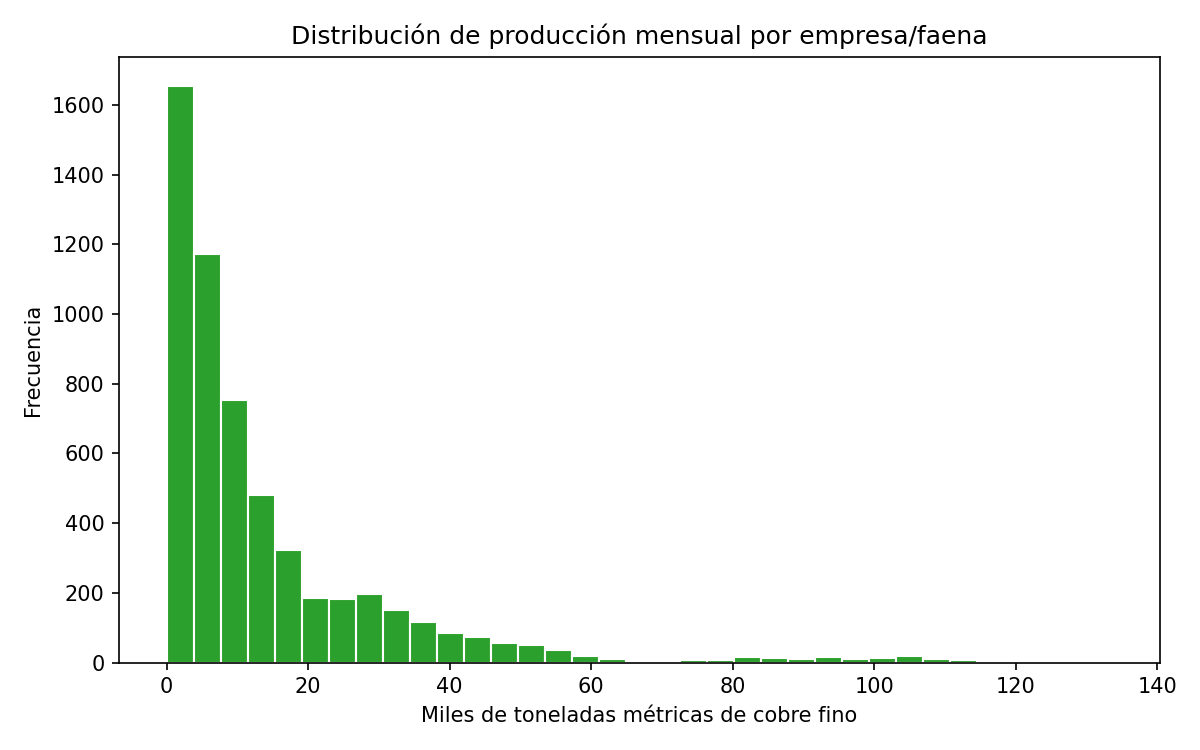
\includegraphics[width=0.93\textwidth]{graficos/hist_empresas_faenas.png}
        };
      \end{tikzpicture}
    \end{column}
    \begin{column}{0.38\textwidth}
      \panel{0.95\textwidth}{
        \textbf{Faenas con mayor promedio mensual positivo}\\[3pt]
        \begin{tabular}{lr}
        \toprule
        Faena & Prom. \\
        \midrule
        Escondida & 95,6 \\
        Chuqui y R. Tomic & 51,3 \\
        Collahuasi & 44,5 \\
        El Teniente & 35,2 \\
        Los Pelambres & 29,0 \\
        \bottomrule
        \end{tabular}\\[6pt]
        Promedio calculado solo en meses con producción positiva. Pocas operaciones grandes explican una parte importante del volumen nacional.
      }
    \end{column}
  \end{columns}
\end{frame}

\begin{frame}[plain]
  \bgphoto{imagenes/escondida.jpg}{carbon}{0.82}
  \copperband
  \vspace{0.32cm}
  \slidetitle{white}{8. Relaciones con la producción nacional}

  \begin{columns}[T,onlytextwidth]
    \begin{column}{0.49\textwidth}
      \begin{tikzpicture}
        \node[rounded corners=5pt, fill=white, inner sep=4pt] {
          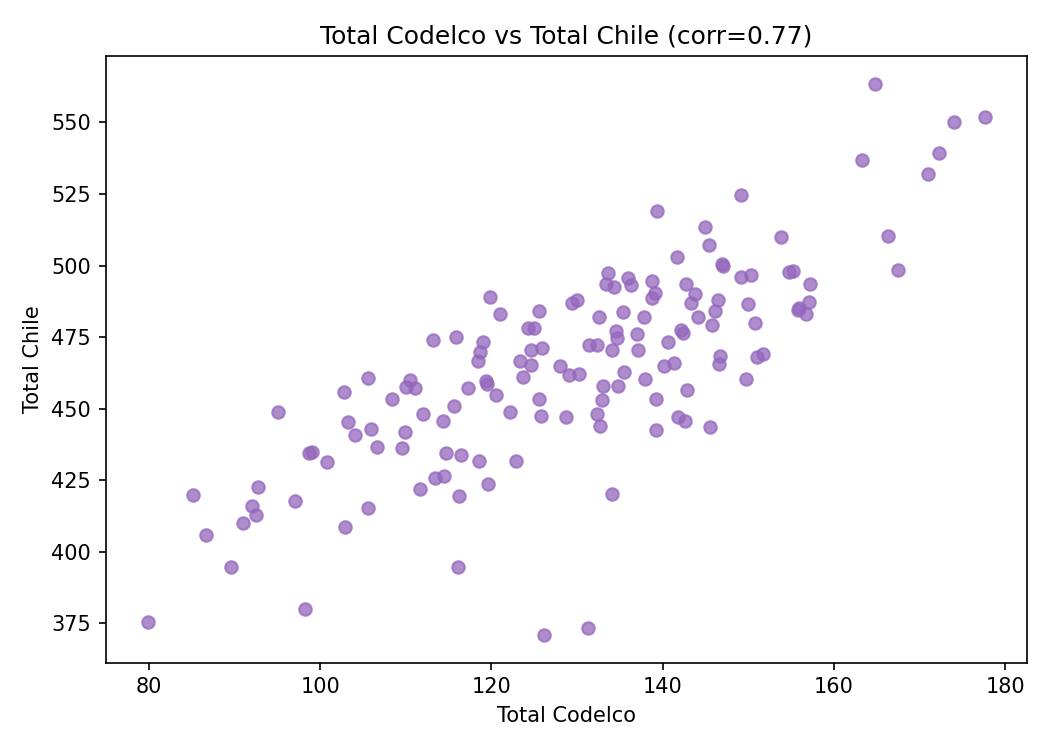
\includegraphics[width=0.94\textwidth]{graficos/scatter_codelco_total_chile.png}
        };
      \end{tikzpicture}
      \vspace{0.08cm}
      \centering{\color{arena}\bfseries Correlación Codelco--Chile: 0,77}
    \end{column}
    \begin{column}{0.49\textwidth}
      \begin{tikzpicture}
        \node[rounded corners=5pt, fill=white, inner sep=4pt] {
          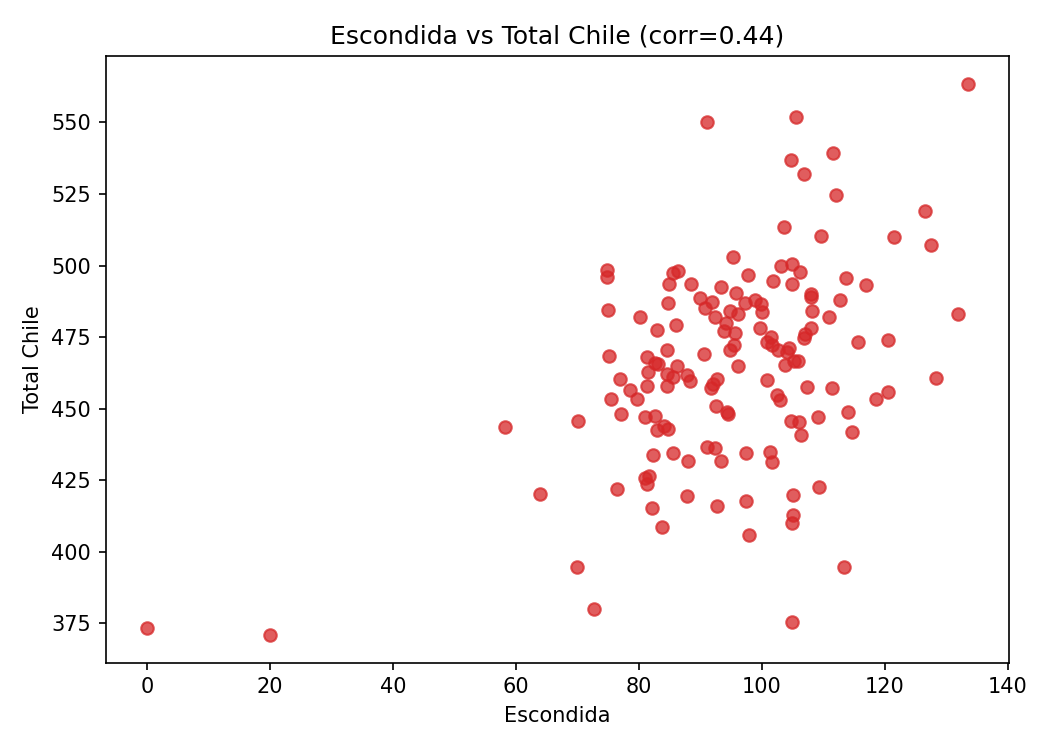
\includegraphics[width=0.94\textwidth]{graficos/scatter_escondida_total_chile.png}
        };
      \end{tikzpicture}
      \vspace{0.08cm}
      \centering{\color{arena}\bfseries Correlación Escondida--Chile: 0,44}
    \end{column}
  \end{columns}

  \vspace{0.18cm}
  \darkpanel{0.96\textwidth}{
    {\color{white}Codelco, como agregado, se mueve más cerca del total nacional que una faena individual, aunque Escondida sea la operación de mayor producción promedio positiva.}
  }
\end{frame}

\begin{frame}[plain]
  \bgphoto{imagenes/catodo_cobre.jpg}{white}{0.84}
  \copperband
  \vspace{0.34cm}
  \slidetitle{mineral}{9. Correlaciones relevantes}

  \begin{columns}[T,onlytextwidth]
    \begin{column}{0.48\textwidth}
      \panel{0.96\textwidth}{
        \textbf{Mayor relación con total\_chile}\\[3pt]
        \scriptsize
        \begin{tabular}{lrl}
        \toprule
        Variable & Corr. & Intensidad \\
        \midrule
        total\_codelco & 0,77 & Alta \\
        chuqui\_y\_r\_tomic & 0,75 & Alta \\
        chuquicamata & 0,71 & Alta \\
        el\_teniente & 0,59 & Media \\
        los\_pelambres & 0,57 & Media \\
        escondida & 0,44 & Media \\
        collahuasi & 0,30 & Baja \\
        \bottomrule
        \end{tabular}
      }
    \end{column}
    \begin{column}{0.48\textwidth}
      \darkpanel{0.96\textwidth}{
        {\color{arena}\bfseries Lectura}\\[4pt]
        {\color{white}\small
        La relación más fuerte aparece en Codelco porque agrupa varias divisiones. En cambio, una faena individual puede ser grande, pero no necesariamente explica sola el movimiento nacional mensual.}
      }
      \vspace{0.22cm}
      \panel{0.96\textwidth}{
        \small Este punto justifica el uso de scatter plots: ambas variables son numéricas y permiten observar asociación, dispersión y meses alejados del patrón.
      }
    \end{column}
  \end{columns}
\end{frame}

\begin{frame}[plain]
  \bgphoto{imagenes/mineral_cobre.jpg}{papel}{0.88}
  \copperband
  \vspace{0.34cm}
  \slidetitle{mineral}{10. Valores faltantes y meses sin dato}

  \begin{columns}[T,onlytextwidth]
    \begin{column}{0.52\textwidth}
      \panel{0.96\textwidth}{
        \textbf{Antes del filtro final}\\[3pt]
        \scriptsize
        \begin{tabular}{lrr}
        \toprule
        Variable & Faltantes & Porcentaje \\
        \midrule
        chuquicamata & 9 & 5,77\% \\
        mantoverde & 9 & 5,77\% \\
        los\_pelambres & 9 & 5,77\% \\
        zaldivar & 9 & 5,77\% \\
        centinela\_sulfuros & 9 & 5,77\% \\
        quebrada\_blanca & 9 & 5,77\% \\
        \bottomrule
        \end{tabular}
      }
    \end{column}
    \begin{column}{0.44\textwidth}
      \darkpanel{0.96\textwidth}{
        {\color{arena}\bfseries Interpretación}\\[4pt]
        {\color{white}\small
        Los faltantes se concentran en meses donde el archivo todavía no informa producción nacional completa. Por eso no se imputan: se filtran los meses con total\_chile igual a cero.}
      }
      \vspace{0.22cm}
      \panel{0.96\textwidth}{
        \small Después de limpiar, el dataset ancho queda con 147 meses, 44 columnas y sin filas duplicadas. El período final usado es enero 2014 a marzo 2026.
      }
    \end{column}
  \end{columns}
\end{frame}

\begin{frame}[plain]
  \bgphoto{imagenes/camion_mina.jpg}{white}{0.84}
  \copperband
  \vspace{0.32cm}
  \slidetitle{mineral}{11. Outliers: no todo valor extremo es error}

  \begin{columns}[T,onlytextwidth]
    \begin{column}{0.52\textwidth}
      \panel{0.95\textwidth}{
        \textbf{Meses detectados por rango intercuartil}\\[3pt]
        \begin{tabular}{lr}
        \toprule
        Mes & Total Chile \\
        \midrule
        Feb. 2017 & 370,8 \\
        Mar. 2017 & 373,1 \\
        Dic. 2018 & 550,1 \\
        Dic. 2019 & 551,8 \\
        Feb. 2023 & 380,0 \\
        Dic. 2024 & 563,6 \\
        Feb. 2026 & 375,4 \\
        \bottomrule
        \end{tabular}
      }
    \end{column}
    \begin{column}{0.43\textwidth}
      \darkpanel{0.95\textwidth}{
        {\color{arena}\bfseries Decisión}\\[4pt]
        {\color{white}Se conservaron estos meses porque pueden representar mantenciones, paralizaciones, cambios operacionales o cierres de periodo. En minería, un outlier puede ser información, no ruido.}
      }
      \vspace{0.22cm}
      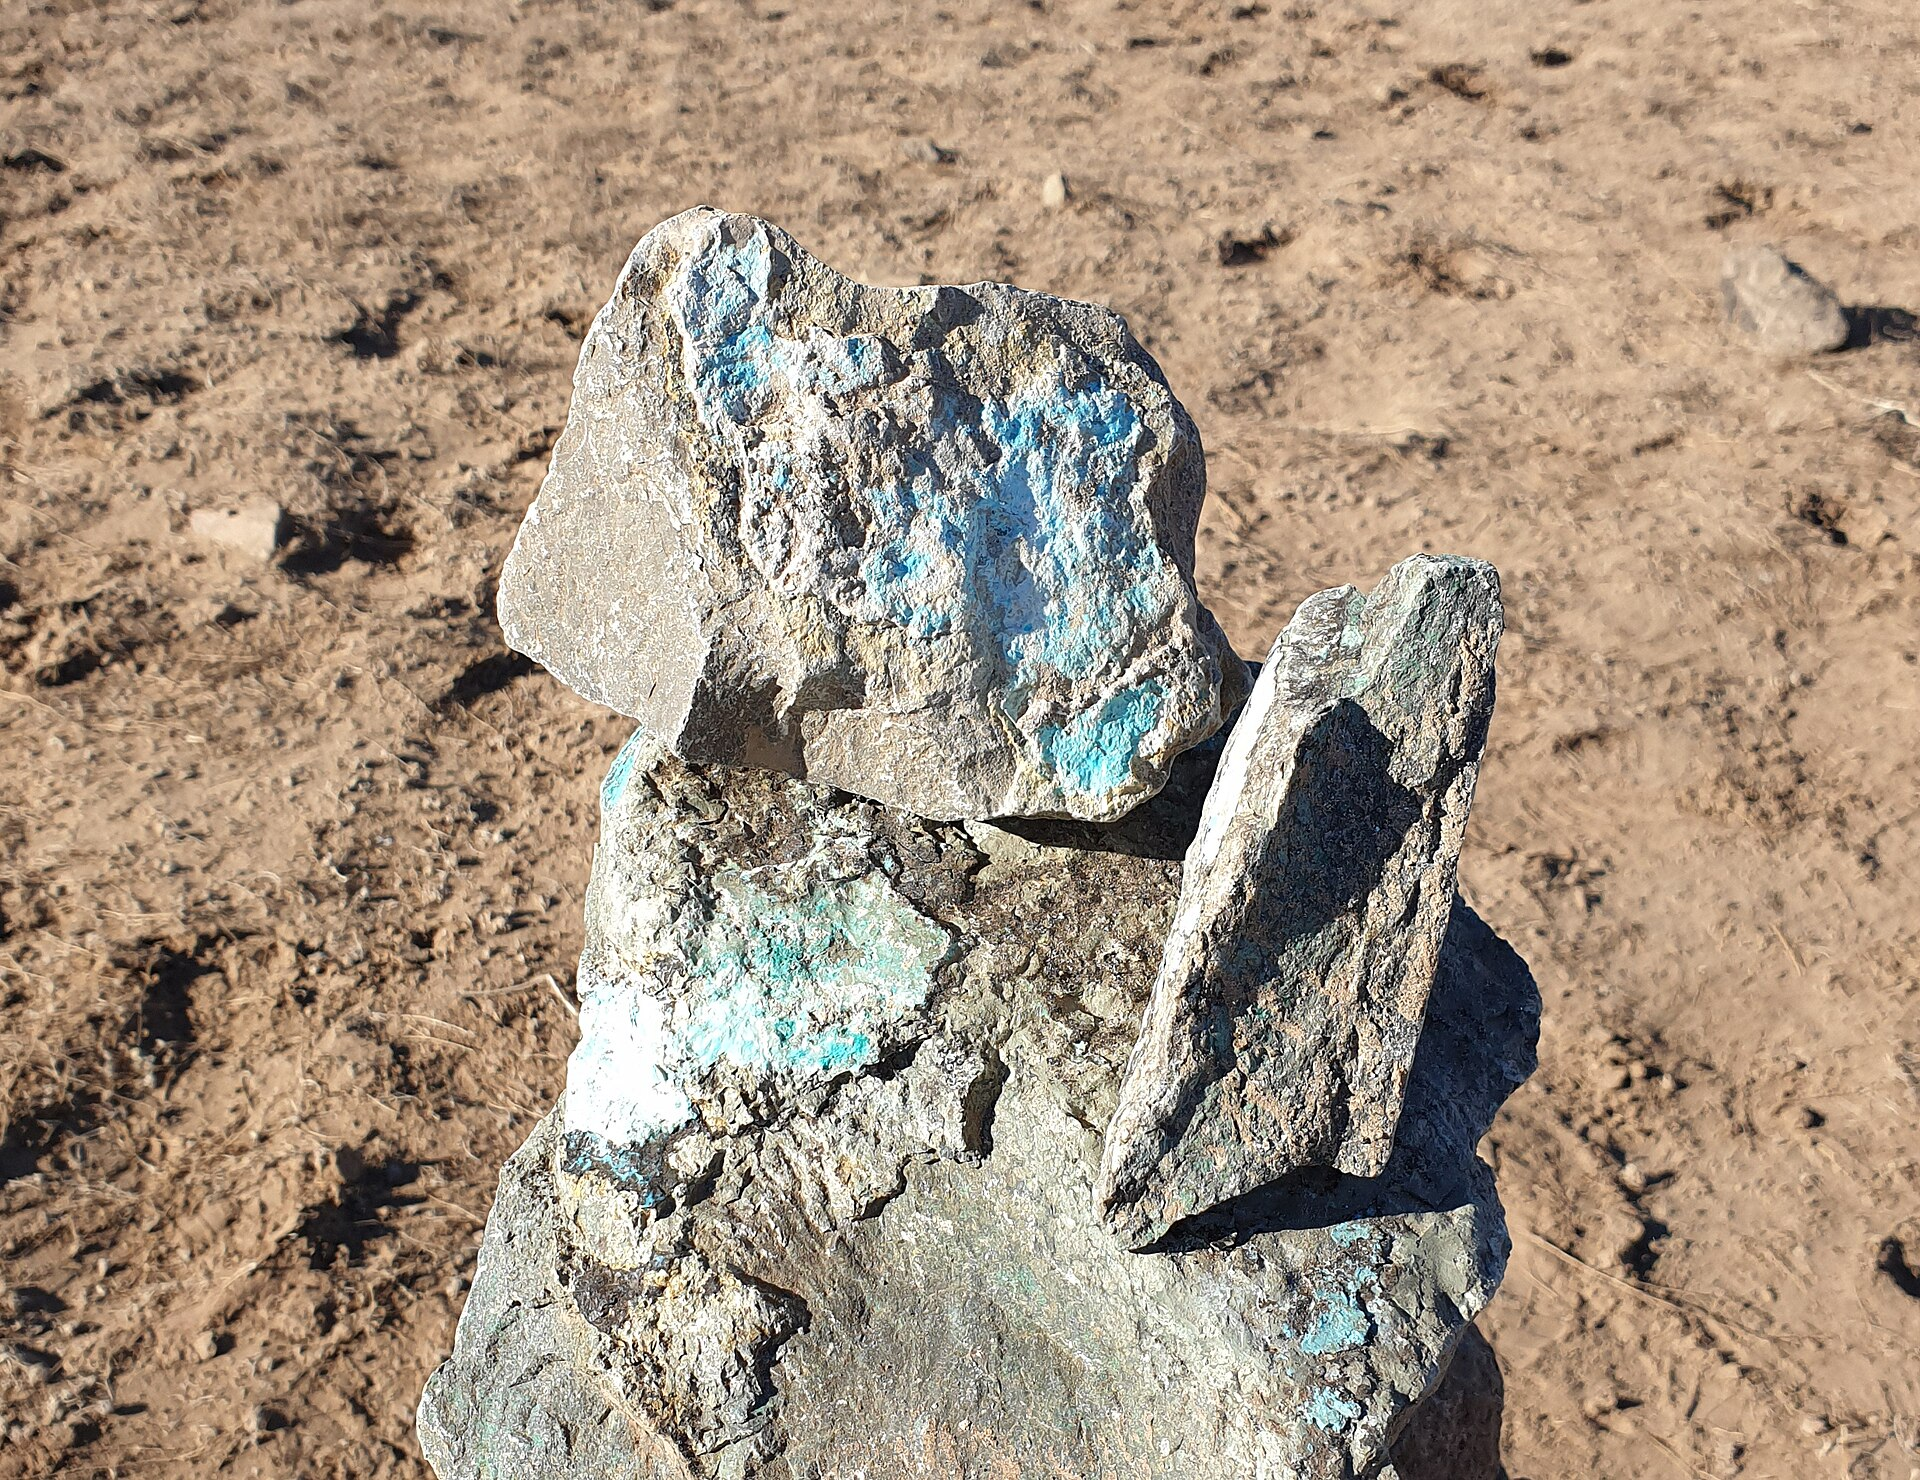
\includegraphics[width=0.95\textwidth,height=0.25\textheight,keepaspectratio]{imagenes/mineral_cobre.jpg}
    \end{column}
  \end{columns}
\end{frame}

\begin{frame}[plain]
  \bgphoto{imagenes/escondida.jpg}{carbon}{0.78}
  \copperband
  \vspace{0.34cm}
  \slidetitle{white}{12. Asimetría y concentración}

  \begin{columns}[T,onlytextwidth]
    \begin{column}{0.50\textwidth}
      \panel{0.96\textwidth}{
        \textbf{Medidas de forma}\\[3pt]
        \scriptsize
        \begin{tabular}{lrr}
        \toprule
        Variable & Asimetría & Curtosis \\
        \midrule
        total\_chile & -0,12 & 0,69 \\
        total\_codelco & -0,13 & -0,29 \\
        escondida & -1,53 & 7,48 \\
        collahuasi & -0,36 & 0,48 \\
        los\_pelambres & -0,76 & 0,91 \\
        el\_teniente & -0,72 & 0,57 \\
        \bottomrule
        \end{tabular}
      }
    \end{column}
    \begin{column}{0.46\textwidth}
      \darkpanel{0.96\textwidth}{
        {\color{arena}\bfseries Resultado clave}\\[4pt]
        {\color{white}\small
        Escondida destaca por asimetría negativa y curtosis alta. Esto indica meses especialmente bajos y presencia de valores extremos, coherente con una faena de gran escala que puede alterar el total nacional cuando se desvía de su nivel habitual.}
      }
      \vspace{0.20cm}
      \panel{0.96\textwidth}{
        \small La decisión fue no imputar ni borrar automáticamente estos valores, sino tratarlos como observaciones relevantes del proceso productivo.
      }
    \end{column}
  \end{columns}
\end{frame}

\begin{frame}[plain]
  \bgphoto{imagenes/catodo_cobre.jpg}{carbon}{0.76}
  \copperband
  \vspace{0.42cm}
  \slidetitle{white}{13. Conclusiones}

  \begin{columns}[T,onlytextwidth]
    \begin{column}{0.52\textwidth}
      \darkpanel{0.96\textwidth}{
        {\color{arena}\large\bfseries Hallazgo central}\\[4pt]
        {\color{white}La producción mensual chilena de cobre es relativamente estable, pero está concentrada en pocas operaciones grandes y presenta meses puntuales que merecen explicación económica u operacional.}
      }
    \end{column}
    \begin{column}{0.42\textwidth}
      \panel{0.95\textwidth}{
        \begin{itemize}
          \item Escondida lidera por producción promedio positiva.
          \item Codelco explica mejor el movimiento del total nacional.
          \item La limpieza fue necesaria por la estructura original del Excel.
          \item El formato largo deja el dataset listo para análisis posteriores.
        \end{itemize}
      }
    \end{column}
  \end{columns}
\end{frame}

\begin{frame}[plain]
  \bgphoto{imagenes/mineral_cobre.jpg}{white}{0.88}
  \copperband
  \vspace{0.35cm}
  \slidetitle{mineral}{14. Fuentes y créditos visuales}

  \panel{0.92\textwidth}{
    \small
    \begin{itemize}
      \item Datos: COCHILCO, ``Producción de Cobre Mina por Empresa Mensual''.
      \item Chuquicamata: Owen Cliffe / Zootalures, Wikimedia Commons, CC BY-SA 3.0.
      \item Escondida: NASA Johnson Space Center / Expedition 22 crew, Wikimedia Commons, dominio público en Estados Unidos.
      \item Cátodo de cobre: WeHaKa, Wikimedia Commons, CC BY-SA 4.0.
      \item Mineral de cobre: S. Rae, Wikimedia Commons, CC BY 2.0.
      \item Camión minero: Phil Whitehouse, Wikimedia Commons, CC BY 2.0.
      \item Gráficos: elaboración propia en Python a partir de COCHILCO.
    \end{itemize}
  }

  \vfill
  \begin{center}
    {\color{cobreoscuro}\LARGE\bfseries Gracias}
  \end{center}
\end{frame}

\end{document}
